\chapter{Results and Analysis} \label{Chap5}

\section{Model Performance Evaluation}
In this section, the outcomes of the Cross-Validation process are presented. This includes a detailed discussion on accuracy, precision, and other relevant metrics specific to financial contexts. The chapter delves into how well the models performed when applied to real-world financial scenarios.

\subsection{Finding Best K-Fold} \label{sec:5.1.1}
\begin{figure}[H]
    \centering
    \includegraphics[width=0.8\textwidth]{figures/jpm/3. Tick Time Gap RSS in Each Folds.png}
    \caption{Tick Time Gap RSS in Each Folds}
    \label{fig:tick_time_gap_rss}
\end{figure}

In this visualization, I present the trend of RSS across different fold values ranging from 0 to 30. The graph clearly illustrates that RSS values are significantly high when the fold value is either very small or very large, aligning with our intuitive understanding. Notably, the RSS reaches its minimum at a fold value of 15. Based on this observation, I set $k=15$ to delve deeper into this problem.

\section{Backtest Results}
Here, the results of the backtesting process are explained, focusing on metrics such as the Harrell Concordance Index (C-Index), Hit Rate (HR), Hit Rate Gap (HRG), and Absolute Maximun Hit Rate Gap (AMG). The section delves into how these metrics performed in evaluating the predictive power of the models in real-world financial scenarios, providing insights into their effectiveness.

\subsection{Harrell Concordance index (C-Index)}
The Harrell Concordance Index (C-Index) is a crucial metric used to assess the predictive power of survival analysis models. It measures the ability of the model to correctly rank the observed durations, indicating how well the model discriminates between different outcomes. Figure \ref{fig:test_concordance_index} present the Concordance Index values for test sets, comparing the outcomes of the Kaplan-Meier Estimator (KM) and Nelson-Aalen Estimator (NA) across various sectors.

\begin{figure}[H]
    \centering
    \includegraphics[width=0.8\textwidth]{figures/jpm/8. Test set concordance index Two Estimators By Sector.png}
    \caption{Test Set Concordance Index of Two Estimators by Sector}
    \label{fig:test_concordance_index}
\end{figure}

In the visualizations \ref{fig:test_concordance_index}, the horizontal axis delineates different sectors, while the vertical axis portrays their respective Concordance Index (C-Index) values. The C-Index, ranging from 0 to 1, serves as a measure of coordination: a value of 1 indicates perfect coordination, while 0 signifies no coordination at all. The histograms represent the average C-Index values across all folds, offering a general overview, while the error bars provide into the variance among the folds, serving as an estimation of the error margin.

Upon observing these visuals, it becomes evident that both the Kaplan-Meier Estimator (KM) and Nelson-Aalen Estimator (NA) exhibit remarkably high C-Index values, approaching almost 1. This suggests a strong coordination between the models, indicating their effective ability to discriminate between different outcomes. Furthermore, the consistency in means and variances across various sectors implies a uniform performance, highlighting the robustness of both estimators across diverse sectors.

However, despite the apparent similarity, it's crucial to note that the C-Index might not capture nuanced differences between the models effectively. The absence of significant disparities in the graphs could stem from the limitations of the C-Index as an indicator. This aspect , exploring the intricacies of the models beyond the C-Index, will be delved into further in Chapter \ref{Chap6}, offering a more comprehensive understanding of their comparative performance.

\subsection{Hit Rate (HR)}
In the following subsection, the Hit Rate (HR) metric is explored, shedding light on the effectiveness of both the Kaplan-Meier Estimator (KM) and Nelson-Aalen Estimator (NA) across various dimensions. Higher HR values indicate a superior predictive ability.

\subsubsection{Overall Hit Rate}
The first set of visuals (Figures \ref{fig:train_hit_rate_overall} and \ref{fig:test_hit_rate_overall}) provides a comprehensive view of the overall HR of both estimators in the training and test sets. These graphs offer insights into how well the models predict outcomes across all data points, highlighting their general performance.

\begin{figure}[H]
    \centering
    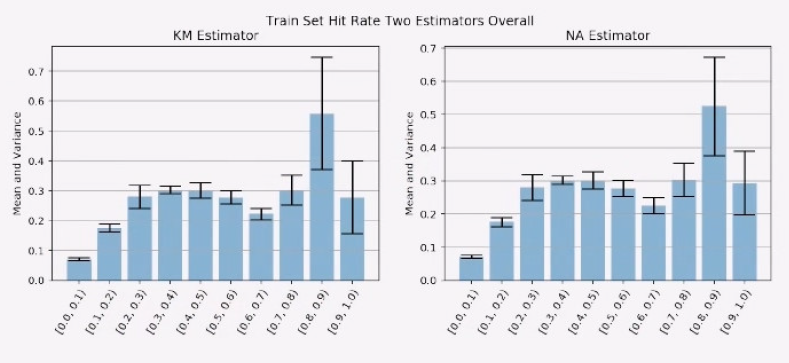
\includegraphics[width=0.8\textwidth]{figures/jpm/10. Train Set Hit Rate Two Estimators Overall.png}
    \caption{Train Set Hit Rate of Two Estimators Overall}
    \label{fig:train_hit_rate_overall}
\end{figure}

\begin{figure}[H]
    \centering
    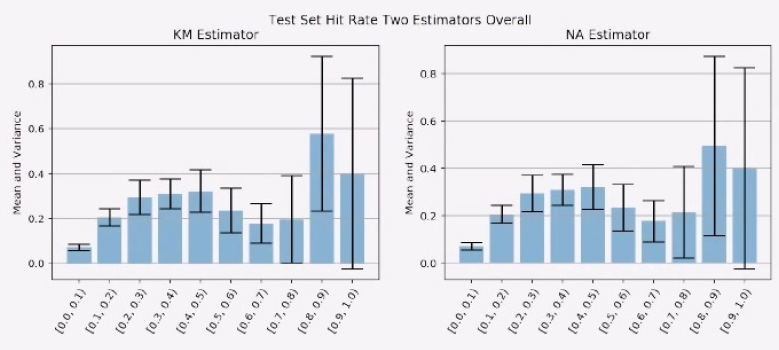
\includegraphics[width=0.8\textwidth]{figures/jpm/12. Test Set Hit Rate Two Estimators Overall.png}
    \caption{Test Set Hit Rate of Two Estimators Overall}
    \label{fig:test_hit_rate_overall}
\end{figure}

The presented graphs, comparing the performance of the Kaplan-Meier Estimator (KM) and Nelson-Aalen Estimator (NA), offer an insightful overview. The x-axis delineates the probability space, segmented into 10 equal intervals, while the y-axis represents the Hit Rate. This analysis amalgamates data from diverse industries, aiming to discern overarching patterns.

In both plots\ref{fig:train_hit_rate_overall} and \ref{fig:test_hit_rate_overall}, both estimators exhibit strikingly similar trends. Across various probability intervals, their means demonstrate comparable distributions. Notably, both estimators show a minor peak between [0.3, 0.4] and a substantial peak between [0.8, 0.9]. The variances, too, display akin patterns, albeit slightly higher within the [0.8, 1] range. Subtle disparities emerge: NA's mean value (0.48) at the [0.8, 0.9] interval in \ref{fig:test_hit_rate_overall} is marginally lower than KM's (0.56). Additionally, NA's variance (0.18) at the [0.7, 0.8] interval in \ref{fig:test_hit_rate_overall} is slightly lower than KM's (0.2).

This analysis underscores the comparable performance and stability of both estimators, affirming their overall consistency. To delve deeper into their distinctions, a more detailed examination is warranted, particularly in dissecting their sector-specific performance, offering valuable insights into their nuanced effectiveness across various sectors. Further scrutiny will shed light on these subtle differences, aiding in a comprehensive evaluation of their predictive capabilities.

\subsubsection{Sector-Specific Hit Rate}
Moving beyond the general overview, the subsequent figures delve into sector-specific analyses. Figures \ref{fig:train_hit_rate_km_sector} and \ref{fig:train_hit_rate_na_sector} focus on the KM and NA estimators' hit rates in the training set, respectively, categorized by different sectors. Similarly, Figures \ref{fig:test_hit_rate_km_sector} and \ref{fig:test_hit_rate_na_sector} provide a sector-wise breakdown for the test set. These visualizations aim to discern if the models exhibit varying predictive accuracies across distinct sectors.

The sector-specific approach enhances my understanding of the models' strengths and weaknesses in different segments of the market, providing valuable insights for strategic decision-making in financial contexts. The ensuing sections will analyze these visualizations, deciphering patterns and drawing conclusions that inform the comparative performance of the KM and NA estimators.

\begin{figure}[H]
    \centering
    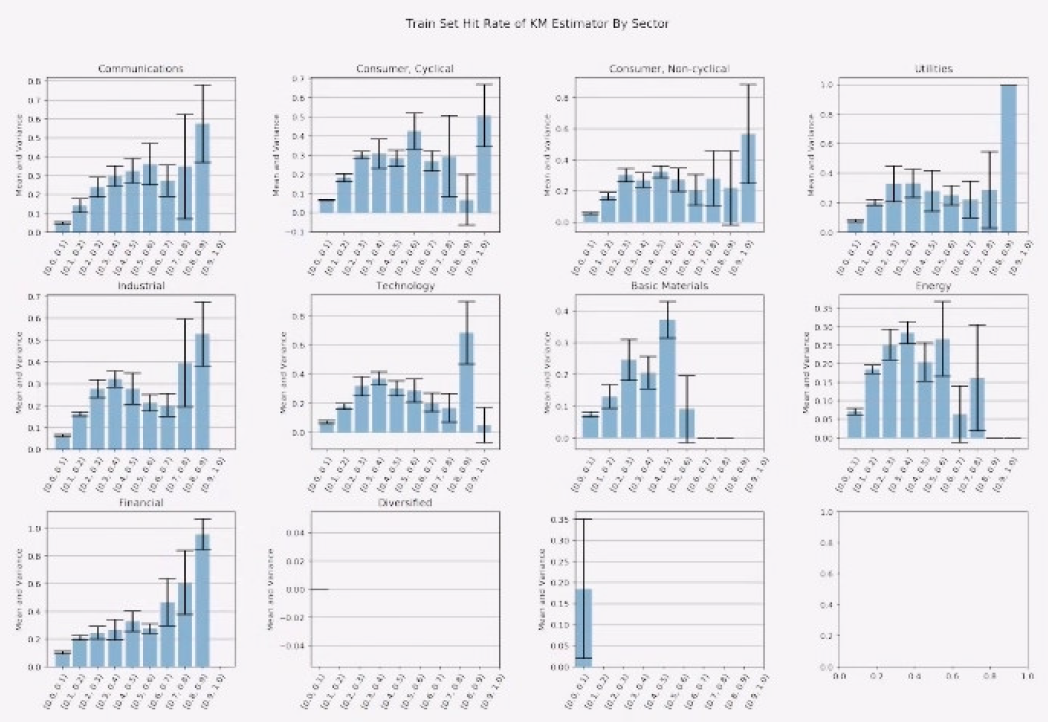
\includegraphics[width=0.8\textwidth]{figures/jpm/14. Train Set Hit Rate of KM Estimator By Sector.png}
    \caption{Train Set Hit Rate of KM Estimator by Sector}
    \label{fig:train_hit_rate_km_sector}
\end{figure}

\begin{figure}[H]
    \centering
    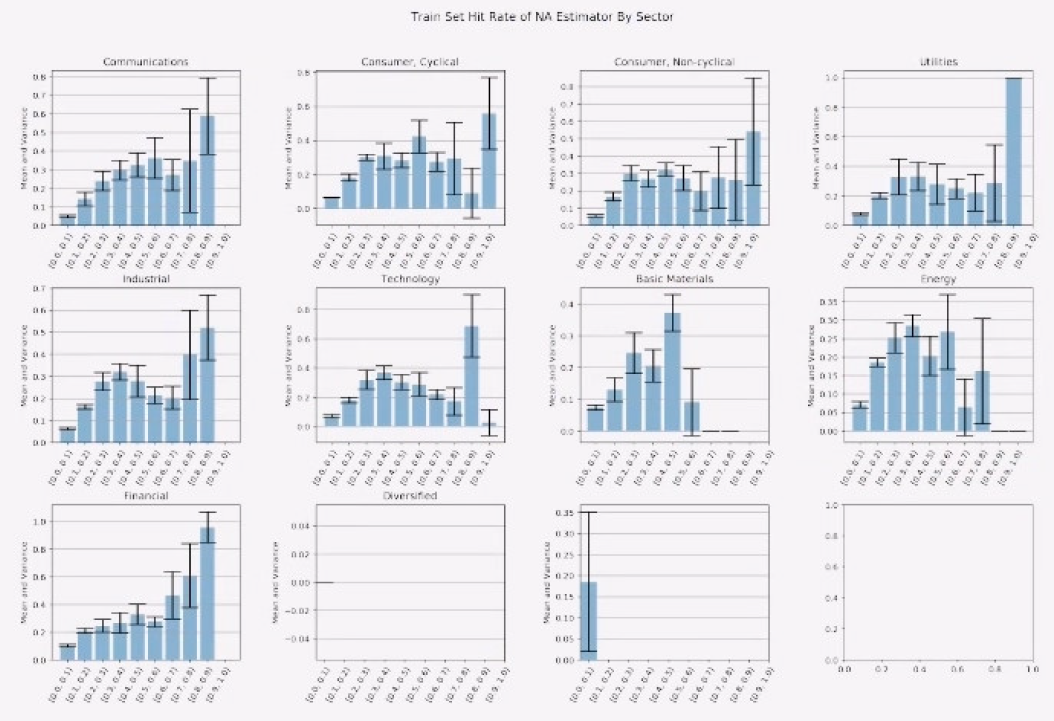
\includegraphics[width=0.8\textwidth]{figures/jpm/15. Train Set Hit Rate of NA Estimator By Sector.png}
    \caption{Train Set Hit Rate of NA Estimator by Sector}
    \label{fig:train_hit_rate_na_sector}
\end{figure}

\begin{figure}[H]
    \centering
    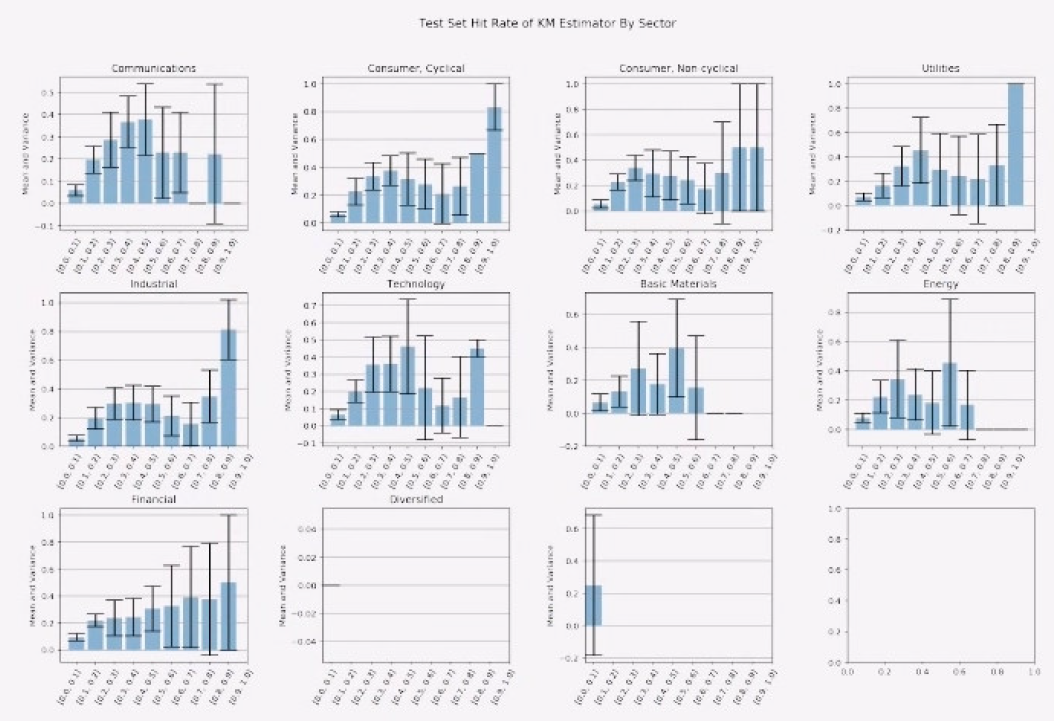
\includegraphics[width=0.8\textwidth]{figures/jpm/16. Test Set Hit Rate of KM Estimator By Sector.png}
    \caption{Test Set Hit Rate of KM Estimator by Sector}
    \label{fig:test_hit_rate_km_sector}
\end{figure}

\begin{figure}[H]
    \centering
    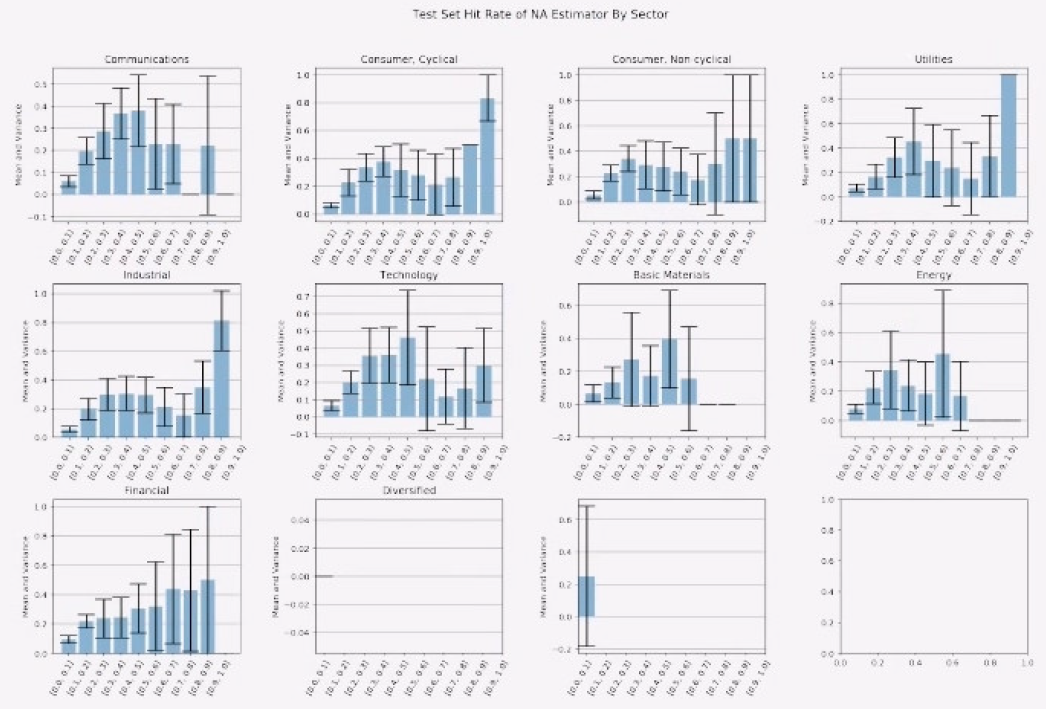
\includegraphics[width=0.8\textwidth]{figures/jpm/17. Test Set Hit Rate of NA Estimator By Sector.png}
    \caption{Test Set Hit Rate of NA Estimator by Sector}
    \label{fig:test_hit_rate_na_sector}
\end{figure}

The presented figures (\ref{fig:train_hit_rate_km_sector} and \ref{fig:train_hit_rate_na_sector} for the train set, and \ref{fig:test_hit_rate_km_sector} and \ref{fig:test_hit_rate_na_sector} for the test set) provide a detailed comparison between the Kaplan-Meier Estimator (KM) and Nelson-Aalen Estimator (NA) across diverse sectors. Each figure is meticulously divided into 12 subplots, corresponding to 11 sectors. Notably, while the initial 9 sectors are sufficiently represented, sectors 10 and 11 exhibit limited data, resulting in numerous empty intervals. Due to the layout constraints, the final subplot remains unoccupied.

Within each subplot, the x-axis delineates the 10 intervals evenly divided by the probability space, while the y-axis represents the Hit Rate. The height of the histogram reflects the average Hit Rate within each fold for the respective sector, with error bars indicating the variance across folds.

In the train set(\ref{fig:train_hit_rate_km_sector} and \ref{fig:train_hit_rate_na_sector}), both estimators exhibit consistent trends. Across diverse probability intervals and sectors, their means demonstrate comparable distributions. Only in the test set(\ref{fig:test_hit_rate_km_sector} and \ref{fig:test_hit_rate_na_sector}), subtle disparities emerge: notably, in the utility sector, KM outperforms NA with a higher mean (0.22) at the [0.6, 0.7] interval, compared to NA's mean of 0.12. Conversely, in the technology sector, KM displays greater stability with a smaller variance (0.05) at the [0.8, 0.9] interval, contrasting NA's variance of 0.23.

These findings reiterate the comparable performance and stability of both estimators (KM and NA). To provide a comprehensive evaluation of their stability, a detailed analysis of their relative errors, specifically the Hit Rate Gap (HRG), will be conducted. Additionally, further exploration of their sector-specific performance will offer valuable insights, enhancing the depth of the analysis.

\subsection{Hit Rate Gap (HRG)}
\subsubsection{Overall Hit Rate Gap}
Figures \ref{fig:train_hit_rate_gap_overall} and \ref{fig:test_hit_rate_gap_overall} present an insightful comparison of Hit Rate Gaps between the Kaplan-Meier Estimator (KM) and Nelson-Aalen Estimator (NA) for the entire dataset, both in the train and test sets. These figures provide a comprehensive overview of the performance disparity between the two estimators.

\begin{figure}[H]
    \centering
    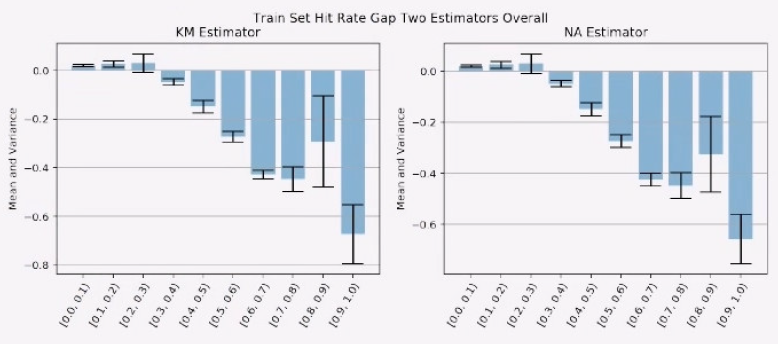
\includegraphics[width=0.8\textwidth]{figures/jpm/11. Train Set Hit Rate Gap Two Estimators Overall.png}
    \caption{Train Set Hit Rate Gap of Two Estimators Overall}
    \label{fig:train_hit_rate_gap_overall}
\end{figure}

\begin{figure}[H]
    \centering
    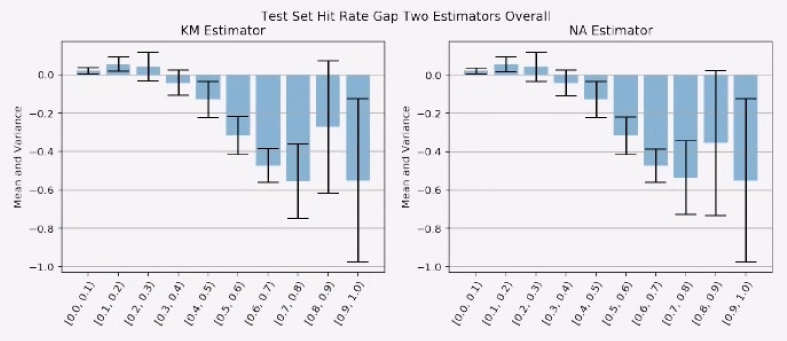
\includegraphics[width=0.8\textwidth]{figures/jpm/13. Test Set Hit Rate Gap Two Estimators Overall.png}
    \caption{Test Set Hit Rate Gap of Two Estimators Overall}
    \label{fig:test_hit_rate_gap_overall}
\end{figure}

In Figures \ref{fig:train_hit_rate_gap_overall} and \ref{fig:test_hit_rate_gap_overall}, the horizontal and vertical coordinates remain consistent with previous representations. The horizontal axis signifies the division of the probability space into ten equal intervals, while the y-axis illustrates the Hit Rate Gap. Most data points lie below the x-axis due to the exceptionally low actual hit rates, hovering around 0.1 (\ref{fig:rfqs_heatmap_real_hr_test}). The expected hit rate estimates steadily increase with the interval endpoints, constituting a monotonic pattern. This analysis amalgamates data from diverse industries, seeking overarching trends amidst the complexity of the financial landscape.

Across both figures, the proximity between the two estimators, KM and NA, persists. Their means exhibit comparable distributions within different probability intervals. Notably, both estimators yield positive values before [0.2, 0.3] and transition to negative values thereafter, reaching a nadir at [0.7, 1.0]. The variances follow a parallel pattern, with \ref{fig:train_hit_rate_gap_overall} showcasing modest variances consistently, while \ref{fig:test_hit_rate_gap_overall} exhibits slightly elevated variances in the range [0.7, 1]. Noteworthy disparities include the mean KM value for the interval [0.8, 0.9] in \ref{fig:train_hit_rate_gap_overall} (-0.29), slightly surpassing NA's mean (-0.32). Similarly, in \ref{fig:test_hit_rate_gap_overall}, the mean KM value (-0.26) for the interval [0.8, 0.9] slightly outperforms NA's mean (-0.34).

\subsubsection{Sector-Specific Hit Rate Gap}
Further granularity is achieved through Figures \ref{fig:train_hit_rate_gap_km_sector}, \ref{fig:train_hit_rate_gap_na_sector}, \ref{fig:test_hit_rate_gap_km_sector}, and \ref{fig:test_hit_rate_gap_na_sector}, which delve into sector-specific analyses. Each of these figures focuses on the Hit Rate Gaps within individual sectors, illuminating the nuanced performance differences between KM and NA across diverse financial sectors.

In these visualizations, the x-axis delineates the 10 intervals evenly divided by the probability space, while the y-axis represents the Hit Rate Gap. The histograms illustrate the average Hit Rate Gap within each fold for the respective sector, offering a detailed glimpse into the disparities in predictive accuracy between the two estimators.

\begin{figure}[H]
    \centering
    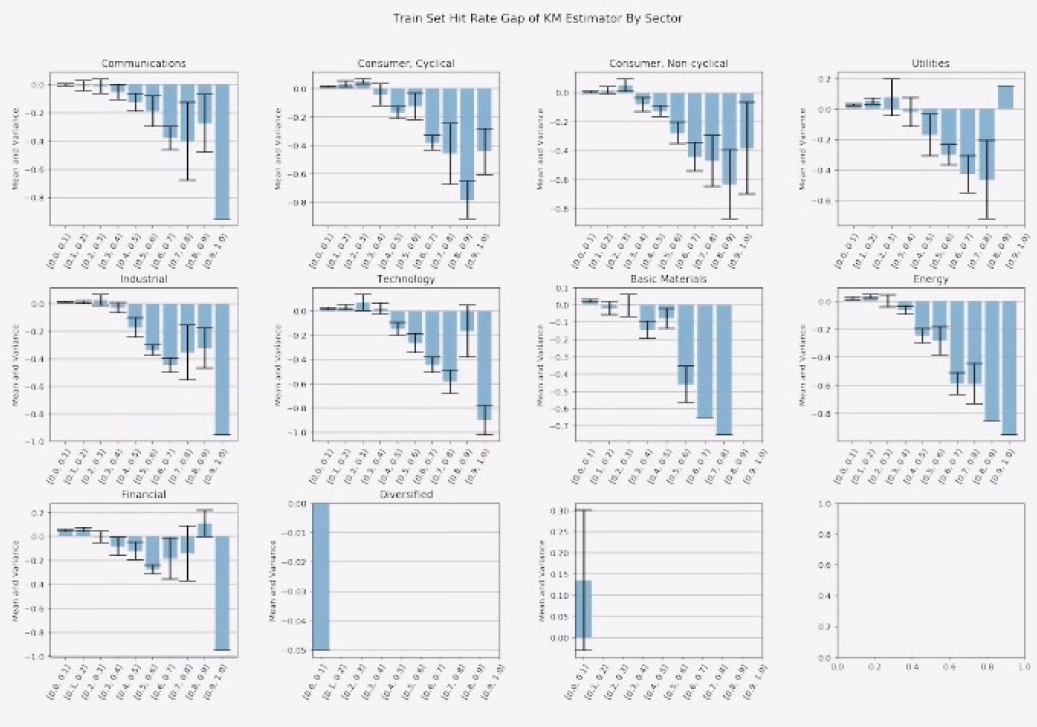
\includegraphics[width=0.8\textwidth]{figures/jpm/18. Train Set Hit Rate Gap of KM Estimator By Sector.png}
    \caption{Train Set Hit Rate Gap of KM Estimator by Sector}
    \label{fig:train_hit_rate_gap_km_sector}
\end{figure}

\begin{figure}[H]
    \centering
    \includegraphics[width=0.8\textwidth]{figures/jpm/19. Train Set Hit Rate Gap of NA Estimator By Sector.png}
    \caption{Train Set Hit Rate Gap of NA Estimator by Sector}
    \label{fig:train_hit_rate_gap_na_sector}
\end{figure}

\begin{figure}[H]
    \centering
    \includegraphics[width=0.8\textwidth]{figures/jpm/20. Test Set Hit Rate Gap of KM Estimator By Sector.png}
    \caption{Test Set Hit Rate Gap of KM Estimator by Sector}
    \label{fig:test_hit_rate_gap_km_sector}
\end{figure}

\begin{figure}[H]
    \centering
    \includegraphics[width=0.8\textwidth]{figures/jpm/21. Test Set Hit Rate Gap of NA Estimator By Sector.png}
    \caption{Test Set Hit Rate Gap of NA Estimator by Sector}
    \label{fig:test_hit_rate_gap_na_sector}
\end{figure}

The depicted histograms (\ref{fig:train_hit_rate_gap_km_sector}, \ref{fig:train_hit_rate_gap_na_sector}, \ref{fig:test_hit_rate_gap_km_sector}, \ref{fig:test_hit_rate_gap_na_sector}) offer a nuanced comparison between the Kaplan-Meier estimator (KM) and the Nelson-Aalen estimator (NA) across diverse sectors. As HR figures above, each figure is meticulously subdivided into 12 sections, corresponding to 11 sectors. Notably, while sectors 1 to 9 provide robust data representation, sectors 10 and 11 exhibit limited data, leading to multiple blank intervals. Due to layout constraints, the final subplot remains vacant.

In each subgraph, the x-axis delineates the probability space across ten intervals, while the y-axis portrays the hit rate gap. The histogram's height signifies the average hit rate within each fold of the respective sector, while the error bars denote the fold-to-fold variance.

Within the training set (\ref{fig:train_hit_rate_gap_km_sector}, \ref{fig:train_hit_rate_gap_na_sector}), both estimators exhibit consistent patterns. With minimal deviations, their mean and variance align in various probability intervals and sectors, underscoring their coherence. However, in the Consumer non-cyclical sector at [0.8, 0.9], KM's mean (-0.62) slightly lags behind NA's (-0.59).

The test set (\ref{fig:test_hit_rate_gap_km_sector}, \ref{fig:test_hit_rate_gap_na_sector}) reveals negligible disparities between the estimators, except in the technology and financial sectors. These sectors feature additional data points in the [0.9, 1] interval, resulting in an extra column in the histogram. Aside from these minor differences, their alignment remains remarkable.

This detailed analysis reaffirms the parallel performance and stability of both estimators, underlining their enduring consistency. To offer a more intuitive understanding of their distinctions, I conducted a sector-wise comparison using their maximum values, visualized through line charts.

\subsection{Absolute Maximun Hit Rate Gap (AMG)}
In this segment, we delve into the evaluation of the absolute maximum hit rate gap between the Kaplan-Meier estimator (KM) and the Nelson-Aalen estimator (NA). The presented figures (\ref{fig:train_max_hit_rate_gap_overall}, \ref{fig:test_max_hit_rate_gap_overall}, \ref{fig:train_max_hit_rate_gap_sector}, \ref{fig:test_max_hit_rate_gap_sector}) portray a comprehensive overview of these gaps, both in the overall dataset and when dissected across different sectors.

\subsubsection{Overall Absolute Maximun Hit Rate Gap}
Starting with the global perspective, Figures \ref{fig:train_max_hit_rate_gap_overall} and \ref{fig:test_max_hit_rate_gap_overall} offer a holistic view of the absolute maximum hit rate gaps in the training and test sets, respectively. These visuals provide insights into the extreme disparities between KM and NA, shedding light on the most significant performance gaps across all sectors.

\begin{figure}[H]
    \centering
    \begin{minipage}{0.48\textwidth}
        \centering
        \includegraphics[width=\textwidth]{figures/jpm/22. Train Set Absolute Max Hit Rate Gap of Two Estimators Overall.png}
        \caption{Train Set Absolute Max Hit Rate Gap of Two Estimators Overall}
        \label{fig:train_max_hit_rate_gap_overall}
    \end{minipage}\hfill
    \begin{minipage}{0.45\textwidth}
        \centering
        \includegraphics[width=\textwidth]{figures/jpm/23. Test Set Absolute Max Hit Rate Gap of Two Estimators Overall.png}
        \caption{Test Set Absolute Max Hit Rate Gap of Two Estimators Overall}
        \label{fig:test_max_hit_rate_gap_overall}
    \end{minipage}
\end{figure}

Figure \ref{fig:train_max_hit_rate_gap_overall} illustrates the comparison of the two estimators on the training set, while Figure \ref{fig:test_max_hit_rate_gap_overall} shows the comparison on the test set. The x-axes of both graphs represent different folds, offering insights into the trends of Absolute Maximum Hit Rate Gap (AMG) changes over time. The y-axes indicate AMG values, where higher values denote greater errors. In both images, the blue line represents Kaplan-Meier (KM) and the orange line represents Nelson-Aalen (NA). Transparency is applied to the lines, ensuring a clear view of their overlap, eliminating any data gaps.

In Figure \ref{fig:train_max_hit_rate_gap_overall}, KM exhibits high AMG values at the 0th and 2nd folds, followed by a steady decrease. Conversely, NA shows elevated AMG only at the 2nd fold, remaining consistently low afterward. Subsequent folds show negligible differences between the two estimators.

Moving to Figure \ref{fig:test_max_hit_rate_gap_overall}, both estimators demonstrate notable fluctuations at different folds, yet their overall trends align closely. The most significant disparity occurs at fold 5, where they differ by a maximum of 0.3. These observations confirm the near indistinguishable nature of the two estimators. To delve deeper, a sector-wise classification was performed to uncover potential nuanced differences in their trends.

\subsubsection{Sector-Specific Absolute Maximun Hit Rate Gap}
Moving to a sector-specific analysis, Figures \ref{fig:train_max_hit_rate_gap_sector} and \ref{fig:test_max_hit_rate_gap_sector} break down these absolute maximum gaps within individual sectors. By dissecting the data in this manner, we can discern whether certain sectors exhibit heightened disparities between the two estimators.

\begin{figure}[H]
    \centering
    \includegraphics[width=0.8\textwidth]{figures/jpm/24. Train Set Absolute Max Hit Rate Gap of Two Estimators By Sector.png}
    \caption{Train Set Absolute Max Hit Rate Gap of Two Estimators by Sector}
    \label{fig:train_max_hit_rate_gap_sector}
\end{figure}

\begin{figure}[H]
    \centering
    \includegraphics[width=0.8\textwidth]{figures/jpm/25. Test Set Absolute Max Hit Rate Gap of Two Estimators By Sector.png}
    \caption{Test Set Absolute Max Hit Rate Gap of Two Estimators by Sector}
    \label{fig:test_max_hit_rate_gap_sector}
\end{figure}

Similar to the Sector-Specific Hit Rate analysis, each graph in this set is divided into 12 sub-graphs representing different industries. The coordinates of each subgraph align with those in Figures \ref{fig:train_max_hit_rate_gap_overall} and \ref{fig:test_max_hit_rate_gap_overall}. Notably, the 10th and 11th subgraphs lack sufficient data points, resulting in incomplete information, and the last subgraph remains unutilized.

Figure \ref{fig:train_max_hit_rate_gap_sector} presents the comparison of the two estimators on the training set, while Figure \ref{fig:test_max_hit_rate_gap_sector} depicts the comparison on the test set.

In these two figures, the trends observed for Kaplan-Meier (KM) and Nelson-Aalen (NA) are strikingly similar, highlighting their consistent performance. However, subtle distinctions emerge: in Figure \ref{fig:train_max_hit_rate_gap_sector}, larger errors are noted in the consumer cyclical, consumer noncyclical, industrial, and technology sectors. Conversely, Figure \ref{fig:test_max_hit_rate_gap_sector} exhibits almost no differences, except for a slight variance observed in the technology and financial sectors.

To meticulously assess the disparities between their distributions, hypothesis testing was employed later to determine whether the means of these distributions are statistically equivalent.

These figures play a pivotal role in deciphering the estimators' relative strengths and weaknesses within distinct sectors, thereby enhancing the comprehensiveness of the analysis. The subsequent sections will delve into a detailed interpretation of these findings, shedding light on the underlying trends and implications for the financial domain.

\section{Hypothesis Test Results}
This section presents the results of the hypothesis tests conducted to compare the performance of the Kaplan-Meier Estimator (KM) and Nelson-Aalen Estimator (NA) overall and within different sectors. The chapter meticulously analyzes the outcomes of these estimators, highlighting significant differences observed in the finance domain.

\begin{table}[H]
    \caption{P-Value - Absolute Max Hit Rate Gap Difference of KM and NA by Sector}
    \label{tab:pvalue_by_sector}
    \centering
    \begin{tabular}{|c|c|}
        \hline
        \textbf{Overall} & 0.55 \\
        \hline
        \textbf{Communications} & 0.99 \\
        \textbf{Consumer, Cyclical} & 0.95 \\
        \textbf{Consumer, Non-cyclical} & 0.64 \\
        \textbf{Utilities} & 1.00 \\
        \textbf{Industrial} & 0.60 \\
        \textbf{Technology} & 0.74 \\
        \textbf{Basic Materials} & 1.00 \\
        \textbf{Energy} & 1.00 \\
        \textbf{Financial} & 1.00 \\
        \textbf{Diversified} & NaN \\
        \textbf{Others} & NaN \\
        \hline
        $\alpha$ Level & 0.05\\
        \hline
    \end{tabular}
\end{table}

\subsection{Overall Comparison}
The overall p-value obtained from the two-sample t-test comparing the mean AMG of KM and NA estimators was 0.55. Since this p-value is greater than the chosen significance level ($\alpha = 0.05$), we fail to reject the null hypothesis. This suggests that there is no significant difference in the mean AMG between KM and NA estimators when considering all sectors collectively.

\subsection{Sector-Specific Comparison}
When comparing the mean AMG by sector, the p-values for various sectors ranged from 0.60 to 1.00. In all sectors, the p-values were greater than the significance level ($\alpha = 0.05$), indicating no statistically significant difference in the mean AMG between KM and NA estimators within any specific sector. Therefore, for each sector, we fail to reject the respective null hypotheses.

\subsection{Conclusion}
In both the overall and sector-specific analyses, the p-values were higher than the chosen significance level ($\alpha = 0.05$), suggesting that there is no significant difference in the mean AMG between the KM and NA estimators. Consequently, based on the provided data and the chosen significance level, there is no statistical evidence to conclude that one estimator performs significantly better than the other in terms of AMG across the examined sectors.

